\clearpage
\section{Detailed Proofs for  \Cref{sec:mechanism}} \label{app:mechanism}
In this section, we work on full attention layers with normalized ReLU activation $\sigma(\cdot) = \frac{1}{n} \mathrm{ReLU}(\cdot)$ given $n$ examples. 
\begin{definition}
\label{def:attn_full_relu}
    A full attention layer with $M$ heads and ReLU activation is also denoted as $\mathrm{Attn}$ on any input sequence $\bH = \begin{bmatrix}
        \bh_1, \cdots, \bh_N
    \end{bmatrix} \in \mathbb R^{D \times N}$, where $D$ is the dimension of hidden states and $N$ is the sequence length. In the vector form,
    \begin{equation}
         \tilde{\bh}_t = [\mathrm{Attn}(\bH)]_t = \bh_t +  \frac{1}{n} \sum_{m=1}^M \sum_{j=1}^n \mathrm{ReLU} \left(\inner{\bQ_m \bh_t, \bK_m \bh_j}\right) \cdot \bV_m \bh_j
    \end{equation}
\end{definition}
\begin{remark}
    This is slightly different from the \textbf{causal} attention layer (see \cref{def:attn}) in that at each time stamp $t$, the attention layer in \cref{def:attn_full_relu} has full information of all hidden states $j \in [n]$, unlike causal attention layer which requires $j \in [t]$. 
\end{remark}

%\subsection{Proof of Lemma \ref{lemma:sum}}

\subsection{Helper Results}

We begin by constructing a useful component for our proof, and state some existing constructions from \citet{Akyrek2022WhatLA}.

\begin{restatable}{lemma}{LemmaSum} \label{lemma:sum}
    Given hidden states $\{\bh_1, \cdots, \bh_n\}$, there exists query, key and value matrices $\bQ, \bK, \bV$ respectively such that one attention layer can compute $\sum_{j=1}^n \bh_j$. 
\end{restatable}
\begin{proof}
We can pad each hidden state by $1$ and $0$'s such that $\bh_t' \leftarrow \begin{bmatrix}
    \bh_t \\ 1 \\ \zero_d
\end{bmatrix} \in \mathbb R^{2d+1}$ . We construct two heads where $\bQ_1 = \bK_1 = \bQ_2 = \begin{bmatrix}
    \bO_{d \times d} & \bO_{d \times 1} & \bO_{d \times d}\\
    \bO_{1 \times d} & 1  & \bO_{1 \times d} \\
    \bO_{d \times d} & \bO_{d \times 1} & \bO_{d \times d}
\end{bmatrix}$ and $\bK_2 = -\bK_1$. Then $\begin{bmatrix}
    \bO_{d \times d} & \bO_{d \times 1} & \bO_{d \times d}\\
    \bO_{1 \times d} & 1  & \bO_{1 \times d} \\
    \bO_{d \times d} & \bO_{d \times 1} & \bO_{d \times d}
\end{bmatrix} \bh_t' = \begin{bmatrix}
    \zero_d \\ 1 \\ \zero_d
\end{bmatrix}$.

Let $\bV_1 = \bV_2 = \begin{bmatrix}
    \bO_{(d+1) \times d} & \bO_{(d+1) \times (d+1)} \\
    n\bI_{d \times d}  &  \bO_{d \times (d+1)}
\end{bmatrix}$ so that $\bV_m \begin{bmatrix}
    \bh_j \\ 1 \\ \zero_d
\end{bmatrix} = \begin{bmatrix}
    \zero_{d+1} \\ n \bh_j 
\end{bmatrix}$. 

We apply one attention layer to these 1-padded hidden states and we have 
\begin{equation}
\begin{aligned}
    \tilde{\bh}_t  & = \bh_t' + \frac{1}{n} \sum_{m=1}^2 \sum_{j=1}^n \mathrm{ReLU} \left(\inner{\bQ_m \bh_t', \bK_m \bh_j'}\right) \cdot \bV_m \bh_j' \\
    &= \bh_t' +  \frac{1}{n} \sum_{j=1}^n \Big[\mathrm{ReLU}(1) + \mathrm{ReLU}(-1)\Big] \cdot \begin{bmatrix}
    \zero_{d+1} \\ n \bh_j 
\end{bmatrix} \\
    &= \begin{bmatrix}
        \bh_t \\ 1 \\ \zero_d
    \end{bmatrix} + 
    \begin{bmatrix}
    \zero_{d+1} \\  \sum_{j=1}^n \bh_j 
\end{bmatrix} = \begin{bmatrix}
        \bh_t \\ 1 \\ \sum_{j=1}^n \bh_j
    \end{bmatrix}
\end{aligned}
\end{equation}  
\end{proof}

%\subsection{Details of Proposition~\ref{prop:akyrek}} 

\begin{proposition}[\citealp{Akyrek2022WhatLA}]\label{prop:akyrek}
    Each of \verb|mov|, \verb|aff|, \verb|mul|, \verb|div|  can be implemented by a single transformer layer. These four operations are mappings $\mathbb R^{D \times N} \rightarrow \mathbb R^{D \times N}$, expressed as follows, 

\verb|mov|$(\bH; s, t, i, j, i', j')$: selects the entries of the $s$-th column of $\bH$ between rows $i$ and $j$, and copies
them into the $t$-th column ($t \geq s$) of $\bH$ between rows $i'$ and $j'$. 

\verb|mul|$(\bH; a, b, c, (i, j), (i', j'), (i'', j''))$: in each column $\bh$ of $\bH$, interprets the entries between $i$ and $j$ as an $a \times b$ matrix $\bA_1$, and the entries between $i'$ and $j'$ as a $b \times c$ matrix $\bA_2$, multiplies these matrices together, and stores the result between rows $i''$ and $j''$, yielding a matrix in which each column has the form 
$\begin{bmatrix}
    \bh_{:i''-1}, \bA_1 \bA_2, \bh_{j'':}
\end{bmatrix}^\top$. This allows the layer to implement inner products. 

\verb|div|$(\bH; (i, j), i', (i'', j''))$: in each column $\bh$ of $\bH$, divides the entries between $i$ and $j$ by the absolute value of the entry at $i'$, and stores the result between rows $i''$ and $j''$, yielding a matrix in which every column has the form $\begin{bmatrix}
    \bh_{:i''-1}, \bh_{i:j} / |\bh_{i'}|, \bh_{j'':}
\end{bmatrix}^\top$.

\verb|aff|$(\bH; (i, j), (i', j'), (i'', j''), \bW_1, \bW_2, \mathbf{b})$: in each column $\bh$ of $\bH$, applies an affine transformation to the entries between $i$ and $j$ and $i'$ and $j'$, then stores the result between rows $i''$ and $j''$, yielding a matrix in which every column has the form $\begin{bmatrix}
    \bh_{:i''-1}, \bW_1 \bh_{i:j} + \bW_2 \bh_{i':j'} + \mathbf{b}, \bh_{j'':}
\end{bmatrix}^\top$. This allows the layer to implement subtraction by setting $\bW_1 = \bI$ and $\bW_2 = -\bI$.


\end{proposition}



%\clearpage
\subsection{Proof of Theorem~\ref{thm:transformers_newton}}
\TransformersNewton*
\begin{proof} We break the proof into parts.

\paragraph{Transformers Implement Initialization $\bT^{(0)}  = \alpha \bS$.} 
Given input sequence $\bH := \{\bx_1, \cdots, \bx_n\}$, with $\bx_i \in \mathbb R^d$,  we first apply the \verb|mov| operations given by Proposition~\ref{prop:akyrek} (similar to \cite{Akyrek2022WhatLA}, we show only non-zero rows when applying these operations):
\begin{equation}
    \begin{bmatrix}
        \bx_1 & \cdots & \bx_n \\
        & & 
    \end{bmatrix} \overset{\mathrm{mov}}{\longrightarrow} \begin{bmatrix}
        \bx_1 & \cdots & \bx_n  \\
        \bx_1 & \cdots & \bx_n 
    \end{bmatrix}
\end{equation}



We call each column after \verb|mov| as $\bh_j$. With an full attention layer, one can construct two heads with query and value matrices of the form $\bQ_1^\top \bK_1 = -\bQ_2^\top \bK_2 = \begin{bmatrix}
    \bI_{d \times d} & \bO_{d \times d} \\
    \bO_{d \times d} & \bO_{d \times d}
\end{bmatrix}$ such that for any $t \in [n]$, we have 
\begin{equation}
    \sum_{m=1}^2 \mathrm{ReLU} \left(\inner{\bQ_m \bh_t, \bK_m \bh_j}\right) = \mathrm{ReLU}(\bx_t^\top \bx_j) +  \mathrm{ReLU}(-\bx_t^\top \bx_j) = \inner{\bx_t, \bx_j}
\end{equation}
Let all value matrices $\bV_m =n \alpha \begin{bmatrix}
    \bI_{d \times d} & \bO_{d \times d} \\
    \bO_{d \times d} & \bO_{d \times d}
\end{bmatrix}$ for some $\alpha \in \mathbb R$. Combining the skip connections, we have 
\begin{equation}
    \tilde{\bh}_t = \begin{bmatrix}
        \bx_t \\ \bx_t
    \end{bmatrix} + \frac{1}{n} \sum_{j=1}^n \inner {\bx_t, \bx_j} n \alpha \begin{bmatrix}
        \bx_j \\ \zero 
    \end{bmatrix}  = \begin{bmatrix}
        \bx_t \\ \bx_t
    \end{bmatrix} + \begin{bmatrix}
       \alpha \left(\sum_{j=1}^n \bx_j \bx_j^\top \right) \bx_t \\ \zero
    \end{bmatrix} = \begin{bmatrix}
        \bx_t + \alpha \bS \bx_t \\ \bx_t
    \end{bmatrix} 
\end{equation}
Now we can use the \verb|aff| operator to make subtractions and then
\begin{equation}
    \begin{bmatrix}
        \bx_t + \alpha \bS \bx_t \\ \bx_t
    \end{bmatrix}  \overset{\mathrm{aff}}{\longrightarrow}\begin{bmatrix}
        (\bx_t + \alpha \bS \bx_t) - \bx_t  \\ \bx_t
    \end{bmatrix}  = \begin{bmatrix}
         \alpha \bS \bx_t \\ \bx_t
    \end{bmatrix}
\end{equation}

We call this transformed hidden states as $\bH^{(0)}$ and denote $\bT^{(0)} = \alpha \bS$:
\begin{equation}
        \bH^{(0)} = \begin{bmatrix}
            \bh_1^{(0)} & \cdots & \bh_n^{(0)}
        \end{bmatrix} = \begin{bmatrix}
            \bT^{(0)} \bx_1 & \cdots & \bT^{(0)} \bx_n \\
            \bx_1 & \cdots & \bx_n
        \end{bmatrix} 
\label{eqn:input_prompt}
\end{equation}
Notice that $\bS$ is symmetric and thereafter $\bT^{(0)}$ is also symmetric.

\paragraph{Transformers implement Newton Iteration.} 
Let the input prompt be the same as \Cref{eqn:input_prompt}, 
    \begin{equation}
        \bH^{(0)} = \begin{bmatrix}
            \bh_1^{(0)} & \cdots & \bh_n^{(0)}
        \end{bmatrix} = \begin{bmatrix}
            \bT^{(0)} \bx_1 & \cdots & \bT^{(0)} \bx_n \\
            \bx_1 & \cdots & \bx_n
        \end{bmatrix} 
    \end{equation}
    We claim that the $\ell$'s hidden states can be of the similar form 
    \begin{equation}
        \bH^{(\ell)} = \begin{bmatrix}
            \bh_1^{(\ell)} & \cdots & \bh_n^{(\ell)}
        \end{bmatrix} = \begin{bmatrix}
            \bT^{(\ell)} \bx_1 & \cdots & \bT^{(\ell)} \bx_n \\
            \bx_1 & \cdots & \bx_n
        \end{bmatrix} 
    \end{equation}
    We prove by induction that assuming our claim is true for $\ell$, we work on $\ell + 1$:

    Let $\bQ_m = \tilde{\bQ}_m \underbrace{\begin{bmatrix}
        \bO_d & -\frac{n}{2} \bI_d \\
        \bO_d & \bO_d 
    \end{bmatrix}}_{\bG} , \bK_m = \tilde{\bK}_m \underbrace{\begin{bmatrix}
        \bI_d & \bO_d \\
        \bO_d & \bO_d 
    \end{bmatrix}}_{\bJ}$ where $\tilde{\bQ}_1^\top \tilde{\bK}_1 : = \bI$, $\tilde{\bQ}_2^\top \tilde{\bK}_2 : = -\bI$ and $\bV_1 = \bV_2 = \underbrace{\begin{bmatrix}
        \bI_d & \bO_d \\
        \bO_d & \bO_d 
    \end{bmatrix}}_{\bJ}$. A 2-head self-attention layer, with ReLU attentions, can be written has 
    \begin{equation}
        \bh_t^{(\ell+1)} = [\mathrm{Attn}(\bH^{(\ell)})]_t = \bh_t^{(\ell)}+ \frac{1}{n} \sum_{m=1}^2 \sum_{j=1}^n \mathrm{ReLU} \left(\inner{\bQ_m \bh_t^{(\ell)}, \bK_m \bh_j^{(\ell)}}\right) \cdot \bV_m \bh_j^{(\ell)}
    \end{equation}
    where 
    \begin{equation}
    \begin{aligned}
        & \sum_{m=1}^2\mathrm{ReLU} \left(\inner{\bQ_m \bh_t^{(\ell)}, \bK_m \bh_j^{(\ell)}}\right) \cdot \bV_m \bh_j^{(\ell)} \\
        &=  \Big[\mathrm{ReLU} \Big((\bG \bh_t^{(\ell)})^\top \underbrace{\tilde{\bQ}_1^\top \tilde{\bK}_1}_{\bI} (\bJ \bh_j^{(\ell)})\Big)  + \mathrm{ReLU} \Big((\bG \bh_t^{(\ell)})^\top \underbrace{\tilde{\bQ}_2^\top \tilde{\bK}_2}_{-\bI} (\bJ \bh_j^{(\ell)})\Big)  \Big] \cdot (\bJ \bh_j^{(\ell)})\\
        &=  \Big[\mathrm{ReLU} ((\bG \bh_t^{(\ell)})^\top (\bJ \bh_j^{(\ell)})) + \mathrm{ReLU} (-(\bG \bh_t^{(\ell)})^\top  (\bJ \bh_j^{(\ell)})) \Big] \cdot  (\bJ \bh_j^{(\ell)})  \\
        &= (\bG \bh_t^{(\ell)})^\top (\bJ \bh_j^{(\ell)}) (\bJ \bh_j^{(\ell)}) \\
        &=  (\bJ \bh_j^{(\ell)}) (\bJ \bh_j^{(\ell)})^\top (\bG \bh_t^{(\ell)})
    \end{aligned} 
    \end{equation}
    Plug in our assumptions that $\bh_j^{(\ell)} = \begin{bmatrix}
        \bT^{(\ell)} \bx_j \\ \bx_j 
    \end{bmatrix}$, we have $\bJ \bh_j^{(\ell)} = \begin{bmatrix}
        \bT^{(\ell)} \bx_j \\ \zero_d 
    \end{bmatrix}$ and $\bG \bh_t^{(\ell)} = \begin{bmatrix}
       -\frac{n}{2} \bx_t \\ \zero_d 
    \end{bmatrix}$, 
    we have 
    \begin{equation}\label{eqn:h_update}
        \begin{aligned}
\bh_t^{(\ell+1)} &= \begin{bmatrix}
        \bT^{(\ell)} \bx_t \\ \bx_t 
    \end{bmatrix} + \frac{1}{n} \sum_{j=1}^n \begin{bmatrix}
        \bT^{(\ell)} \bx_j \\ \zero_d 
    \end{bmatrix} \begin{bmatrix}
        \bT^{(\ell)} \bx_j \\ \zero_d 
    \end{bmatrix}^\top  \begin{bmatrix}
         -\frac{n}{2} \bx_t \\ \zero_d 
    \end{bmatrix} \\
    &= \begin{bmatrix}
        \bT^{(\ell)} \bx_t - \frac{1}{2} \sum_{j=1}^n  (\bT^{(\ell)} \bx_j) (\bT^{(\ell)} \bx_j)^\top  \bx_t \\ \bx_t  
    \end{bmatrix} \\
    &= \begin{bmatrix}
        \bT^{(\ell)} \bx_t - \frac{1}{2} \bT^{(\ell)} \left(\sum_{j=1}^n \bx_j  \bx_j^\top\right)  {\bT^{(\ell)}}^\top \bx_t \\ \bx_t  
    \end{bmatrix} \\
    &= \begin{bmatrix}
        \left(\bT^{(\ell)} - \frac{1}{2} \bT^{(\ell)} \bS {\bT^{(\ell)}}^\top \right) \bx_t \\ \bx_t 
    \end{bmatrix}
        \end{aligned}
    \end{equation} 
    Now we pass over an MLP layer with
    \begin{equation}
        \bh_t^{(\ell+1)} \leftarrow \bh_t^{(\ell+1)} + \begin{bmatrix}
            \bI_d & \bO_d \\ 
            \bO_d & \bO_d 
        \end{bmatrix} \bh_t^{(\ell+1)} = \begin{bmatrix}
        \left(2\bT^{(\ell)} -  \bT^{(\ell)} \bS {\bT^{(\ell)}}^\top \right) \bx_t \\ \bx_t 
    \end{bmatrix}
    \end{equation}
    Now we denote the iteration
    \begin{equation}
        \bT^{(\ell+1)} = 2\bT^{(\ell)} -  \bT^{(\ell)} \bS {\bT^{(\ell)}}^\top
    \end{equation}
    We find that ${\bT^{(\ell+1)}}^\top =  \bT^{(\ell+1)}$ since $ \bT^{(\ell)}$ and $\bS$ are both symmetric. It reduces to 
    \begin{equation}
        \bT^{(\ell+1)} = 2\bT^{(\ell)} -  \bT^{(\ell)} \bS {\bT^{(\ell)}}
    \end{equation}
    This is exactly the same as the Newton iteration. 


\paragraph{Transformers can implement $\hat{\bw}_\ell^\mathrm{TF} = \bT^{(\ell)} \bX^\top \by$.}
Going back to the empirical prompt format $\{\bx_1, y_1, \cdots, \bx_n, y_n\}$. We can let parameters be zero for positions of $y$'s and only rely on the skip connection up to layer $\ell$, and the $\bH^{(\ell)}$ is then $\begin{bmatrix}
           \bT^{(\ell)} \bx_j & \zero  \\
            \bx_j &  \zero \\
            0 & y_j
        \end{bmatrix}_{j=1}^n $. We again apply operations from Proposition~\ref{prop:akyrek}:
\begin{equation}
    \begin{bmatrix}
           \bT^{(\ell)} \bx_j & \zero  \\
            \bx_j &  \zero \\
            0 & y_j
        \end{bmatrix}_{j=1}^n \overset{\mathrm{mov}}{\longrightarrow} \begin{bmatrix}
           \bT^{(\ell)} \bx_j & \bT^{(\ell)} \bx_j  \\
            \bx_j & \zero \\
            0 & y_j
        \end{bmatrix}_{j=1}^n \overset{\mathrm{mul}}{\longrightarrow} \begin{bmatrix}
            \bT^{(\ell)} \bx_j & \bT^{(\ell)}\bx_j  \\
             \bx_j & \zero \\
             0 & y_j \\
        \zero & \bT^{(\ell)} y_j \bx_j 
        \end{bmatrix}_{j=1}^n 
\label{eqn:Tyjxj}
\end{equation}
Now we apply \Cref{lemma:sum} over all even columns in \Cref{eqn:Tyjxj} and we have 
\begin{equation}
    \mathrm{Output} = \sum_{j=1}^n \begin{bmatrix}
         \bT^{(\ell)}\bx_j \\ \zero \\ y_j \\  \bT^{(\ell)} y_j \bx_j 
    \end{bmatrix} = \begin{bmatrix}
        \bxi \\ \bT^{(\ell)} \sum_{j=1}^n y_j \bx_j 
    \end{bmatrix} = \begin{bmatrix}
        \bxi \\ \bT^{(\ell)} \bX^\top \by 
    \end{bmatrix}
\end{equation}
where $\bxi$ denotes irrelevant quantities. Note that the resulting $\bT^{(\ell)} \bX^\top \by $ is also the same as \newton's predictor $\hat{\bw}_k = \bM_k \bX^\top \by$ after $k$ iterations. We denote $\hat{\bw}_\ell^\mathrm{TF} = \bT^{(\ell)} \bX^\top \by$.

\paragraph{Transformers can make predictions on $\bx_{test}$ by $\inner{\hat{\bw}_\ell^\mathrm{TF}, \bx_\mathrm{test}}$.} 

Now we can make predictions on text query $\bx_\mathrm{test}$:
\begin{equation}
    \begin{bmatrix}
        \bxi &  \bx_\mathrm{test} \\
        \hat{\bw}_\ell^\mathrm{TF} & \bx_\mathrm{test}
    \end{bmatrix} \overset{\mathrm{mov}}{\longrightarrow} \begin{bmatrix}
        \bxi &  \bx_\mathrm{test} \\
        \hat{\bw}_\ell^\mathrm{TF} & \bx_\mathrm{test} \\
        \zero & \hat{\bw}_\ell^\mathrm{TF}
    \end{bmatrix} \overset{\mathrm{mul}}{\longrightarrow} \begin{bmatrix}
        \bxi &  \bx_\mathrm{test} \\
        \hat{\bw}_\ell^\mathrm{TF} & \bx_\mathrm{test} \\
        \zero & \hat{\bw}_\ell^\mathrm{TF} \\
        0 & \inner{\hat{\bw}_\ell^\mathrm{TF}, \bx_\mathrm{test}}
    \end{bmatrix}
\end{equation}

Finally, we can have an readout layer $\bbeta_\mathrm{ReadOut} = \{\bu, v\}$ applied (see \cref{def:readout}) with $\bu = \begin{bmatrix}
    \zero_{3d} & 1 
\end{bmatrix}^\top$ and $v = 0$ to extract the prediction $ \inner{\hat{\bw}_\ell^\mathrm{TF}, \bx_\mathrm{test}}$ at the last location, given by $\bx_\mathrm{test}$. This is exactly how \newton\ makes predictions. 

\paragraph{To Perform $k$ steps of Newton's iterations, Transformers need $\mathcal O(k)$ layers.}

Let's count the layers:
\begin{itemize}
    \item \textbf{Initialization}: \verb|mov| needs $\mathcal O(1)$ layer; gathering $\alpha \bS$ needs $\mathcal O(1)$ layer; and \verb|aff| needs $\mathcal O(1)$ layer. In total, Transformers need $\mathcal O(1)$ layers for initialization. 
    \item \textbf{Newton Iteration}: each exact Newton's iteration requires $\mathcal O(1)$ layer. Implementing $k$ iterations requires $\mathcal O(k)$ layers.
    \item \textbf{Implementing $\hat{\bw}_\ell^\mathrm{TF}$}: We need one operation of \verb|mov| and \verb|mul| each, requiring $\mathcal O(1)$ layer each. Apply \Cref{lemma:sum} for summation also requires $\mathcal O(1)$ layer. 
    \item \textbf{Making prediction on test query}:  We need one operation of \verb|mov| and \verb|mul| each, requiring $\mathcal O(1)$ layer each.
\end{itemize}
Hence, in total, Transformers can implement $k$-step \newton\ and make predictions accordingly using $\mathcal{O}(k)$ layers. 
\end{proof}

{
\begin{remark}
We note that \cite{pmlr-v202-giannou23a} used 13 layers to compute one Newton Iteration, and in our construction, we need only one Transformer layer (with one attention layer and one MLP layer) to compute one Newton Iteration. At the same time, we didn’t use \cite{Akyrek2022WhatLA} for constructing Newton Iterations. \cite{Akyrek2022WhatLA} is applied to initialize Newton and for reading out the prediction. 

In our construction, only the initialization and read-out prediction components use causal attention and softmax because \cite{Akyrek2022WhatLA}'s construction is applied. To be more specific, those are the first 3 layers in initializing Iterative Newton and the last 5 layers in reading out the predictions from the computed pseudo-inverse. All the layers corresponding to the Iterative Newton updates are using full attention and normalized ReLU activations.
\end{remark}

}

{
\begin{remark}
\label{rmk:causal}
We note that our proof can be extended to causal attention for $n$ sufficiently larger than $d$. Under causal attention (see \Cref{def:attn}) with normalized ReLU activation, \Cref{eqn:h_update} can be rewritten as follows, given $t > d$, we first choose $\bG = \begin{bmatrix}
        \bO_d & -\frac{1}{2} \bI_d \\
        \bO_d & \bO_d 
    \end{bmatrix}$, where the coefficient on the upper right block is $-\frac{1}{2}$ instead of $-\frac{n}{2}$ originally. Then
\begin{equation}
    \begin{aligned}
        \bh_t^{(\ell+1)} &= \begin{bmatrix}
        \bT^{(\ell)} \bx_t \\ \bx_t 
    \end{bmatrix} + \frac{1}{t} \sum_{j=1}^t \begin{bmatrix}
        \bT^{(\ell)} \bx_j \\ \zero_d 
    \end{bmatrix} \begin{bmatrix}
        \bT^{(\ell)} \bx_j \\ \zero_d 
    \end{bmatrix}^\top  \begin{bmatrix}
         -\frac{1}{2} \bx_t \\ \zero_d 
    \end{bmatrix} \\
    &= \begin{bmatrix}
        \bT^{(\ell)} \bx_t - \frac{1}{2}~ \frac{1}{t}\sum_{j=1}^t  (\bT^{(\ell)} \bx_j) (\bT^{(\ell)} \bx_j)^\top  \bx_t \\ \bx_t  
    \end{bmatrix} \\
    &= \begin{bmatrix}
        \bT^{(\ell)} \bx_t - \frac{1}{2} \bT^{(\ell)} \left(\frac{1}{t}\sum_{j=1}^t \bx_j  \bx_j^\top\right)  {\bT^{(\ell)}}^\top \bx_t \\ \bx_t  
    \end{bmatrix} \\
    &= \begin{bmatrix}
        \left(\bT^{(\ell)} - \frac{1}{2} \bT^{(\ell)} \hat{\bSigma} {\bT^{(\ell)}}^\top \right) \bx_t \\ \bx_t 
    \end{bmatrix}
    \end{aligned}
\end{equation}
where $\hat{\bSigma} = \frac{1}{t}\sum_{j=1}^t \bx_j  \bx_j^\top$ is the estimate of the covariance matrix given seen in-context examples $\{\bx_j, y_j\}_{j=1}^t$ so far. Since $t > d$, $\hat{\bSigma}$ is an unbiased estimate for $\bSigma \approx \frac{1}{n} \bS$ if $n$ is sufficiently large. The rest of the proof follows similarly, up to the perturbation introduced by the error in the estimate of $\hat{\bSigma}$. 

We also note when $t < d$, the estimate  $\hat{\bSigma} = \frac{1}{t}\sum_{j=1}^t \bx_j  \bx_j^\top$ is no longer a valid covariance matrix since it's singular. Then this gives different $\bT^{(\ell+1)}$ for different time stamp $t < d$ and such error may propagate in our proof. Hence, a formal extension to causal models requires extensive analysis of the error bounds and it is beyond the scope of this work. Nonetheless, we provide a plausible direction of such an extension. 
    
\end{remark}
}



%\section{Generalizations to Sum of Moments Method} \label{app:som}
\subsection{\newton\ as a Sum of Moments Method}\label{sec:newton_moment}
Recall that \newton's method finds $\bS^\dagger$ as follows 
\begin{equation}
    \bM_0 = \underbrace{\frac{2}{\|\bS\bS^\top\|_2}}_{\alpha} ~ \bS^\top, \qquad \bM_k = 2 \bM_{k-1} - \bM_{k-1} \bS \bM_{k-1}, \forall k \geq 1.
\end{equation}

We can expand the iterative equation to moments of $\bS$ as follows. 

\begin{equation}
    \begin{aligned}
        \bM_1 &= 2 \bM_0 - \bM_0 \bS \bM_0  = 2 \alpha \bS^\top - 4 \alpha^2 \bS^\top \bS \bS^\top = 2 \alpha \bS - 4 \alpha^2 \bS^3 .
    \end{aligned}
\end{equation}


Let's do this one more time for $\bM_2$.
\begin{equation}
    \begin{aligned}
        \bM_2 &= 2 \bM_{1} - \bM_{1} \bS \bM_{1} = 2 (2 \alpha \bS - 4 \alpha^2 \bS^3) - (2 \alpha \bS - 4 \alpha^2 \bS^3) \bS (2 \alpha \bS - 4 \alpha^2 \bS^3) \\
        &= 4 \alpha \bS - 8 \alpha^2 \bS^3 - 4 \alpha^2 \bS^3 + 16 \alpha^3 \bS^5 - 16\alpha^4 \bS^7 \\
        &= 4 \alpha \bS - 12 \alpha^2 \bS^3  + 16 \alpha^3 \bS^5 - 16\alpha^4 \bS^7.
    \end{aligned}
\end{equation}

We can see that $\bM_k$ are  summations of moments of $\bS$, with respect to some pre-defined coefficients from the Newton's algorithm. Hence \newton\ is a special of an algorithm which computes an approximation of the inverse using second-order moments of the matrix, 
%In generalizing Newton, we can replace these coefficients as $\beta_j$ corresponding to the $j$-th moment of $\bS$. Note the highest order of $\bS$ grows exponentially over the number of Newton iterations $k$. It's natural to extend the Iterative Newton's method to 
\begin{equation}
    \bM_k = \sum_{s=1}^{2^{k+1} - 1} \beta_s \bS^s
\label{eqn:som}
\end{equation}
with coefficients $\beta_s \in \mathbb R$.

We note that Transformer circuits can represent other sum of moments other than Newton's method. We can introduce different coefficients $\beta_i$ than in the proof of Theorem \ref{thm:transformers_newton} by scaling the value matrices or through the MLP layers. 

\iffalse

\subsection{Transformers Can Implement Sum of Moments Method}
Transformers can implement similar sum of moments method as \Cref{eqn:som}. 
\begin{theorem}\label{thm:tf_som}
    An $L$-layer Transformer can implement the sum of moments method: $\displaystyle \hat{\bw} = \left(\sum_{s=1}^{C_{L}} \beta_s \bS^s\right) \bX^\top \by$, where the highest order of moments $C_L = \frac{1}{2} \left(3^L - 1\right)$.
\end{theorem}

To prove that we begin with a simple lemma:

\begin{lemma}
  \label{lemma:inner_product}
    Given hidden states $\{\bh_1, \cdots \bh_n\}$, there exists query, key and value matrices $\bQ_m, \bK_m, \bV_m$, respectively, so that an attention layer can derive output hidden states $\tilde{\bh}_t = \bh_t +\sum_{j=1}^n \inner {\bh_t, \bh_j} \bh_j$ for all $t \in [n]$. It requires at most 2 heads.   
\end{lemma}
\begin{proof}
        Let $\bQ_1^\top \bK_1 : = \bI$, $\bQ_2^\top \bK_2 : = -\bI$ and $\bV_1 = \bV_2 = n\bI$. A 2-head self-attention layer, with ReLU attentions, can be written has 
    \begin{equation}
    \begin{aligned}
        \tilde{\bh}_t &= [\mathrm{Attn}(\bH)]_t = \bh_t + \frac{1}{n} \sum_{m=1}^2 \sum_{j=1}^n \mathrm{ReLU} \left(\inner{\bQ_m \bh_t, \bK_m \bh_j}\right) \cdot \bV_m \bh_j \\
        &= \bh_t + \frac{1}{n} \sum_{j=1}^n \Big[\mathrm{ReLU} (\bh_t^\top \underbrace{\bQ_1^\top \bK_1}_{\bI} \bh_j) \cdot n\bI \bh_j  + \mathrm{ReLU} (\bh_t^\top \underbrace{\bQ_2^\top \bK_2}_{-\bI} \bh_j) \cdot n\bI \bh_j  \Big] \\
        &= \bh_t + \sum_{j=1}^n \Big[\mathrm{ReLU} (\bh_t^\top \bh_j) + \mathrm{ReLU} (-\bh_t^\top  \bh_j) \Big] \cdot  \bh_j   \\
        &= \bh_t +  \sum_{j=1}^n \inner{\bh_t, \bh_j} \cdot \bh_j  
    \end{aligned} 
    \end{equation}
\end{proof}
\subsubsection{Proof of Theorem~\ref{thm:tf_som}}
\begin{proof}
Recall the form given by Lemma~\ref{lemma:inner_product}:
    \begin{equation}
        \bh_t^{(\ell)} = \bh_t^{(\ell-1)} + \sum_{j=1}^n \inner{\bh_t^{(\ell-1)}, \bh_j^{(\ell-1)}} \cdot \bh_j^{(\ell-1)}
    \label{eqn:tf_iteration}
    \end{equation}
    
We prove by induction. 
Let $\bh_j^{(0)} = \bx_j$ for all $j \in [n]$ and $\bh_t^{(0)} = \bx_t$. Put in \cref{eqn:tf_iteration}, we have
\begin{equation}
\begin{aligned}
    \bh_t^{(1)} &= \bh_t^{(0)} + \sum_{j=1}^n \inner{\bh_t^{(0)}, \bh_j^{(0)}} \cdot \bh_j^{(0)} = \bx_t +  \sum_{j=1}^n \inner{\bx_t, \bx_j} \cdot \bx_j \\
    &= \bx_t + \bS \bx_t = (\bI + \bS) \bh_t^{(0)}
\end{aligned}
\end{equation}
This is equivalent to 
\begin{equation}
    \bH^{(1)} = (\bI + \bS) \bH^{(0)}
\end{equation}

Now suppose $\displaystyle \bH^{(\ell)} = \underbrace{\left(\sum_{s=1}^{C_\ell} \beta_s^{(\ell)} \bS^s\right)}_{\bT^{(\ell)}}\bH^{(0)}$. This implies that 
$\bh_j^{(\ell)} = \bT^{(\ell)} \bh_j^{(0)} = \bT^{(\ell)} \bx_j$ for all $j$. We work on the induction step,
\begin{equation}
\begin{aligned}
    \bh_t^{(\ell+1)} &= \bh_t^{(\ell)} + \sum_{j=1}^n \inner{\bh_t^{(\ell)}, \bh_j^{(\ell)}} \cdot \bh_j^{(\ell)}  = \bh_t^{(\ell)} + \left(\sum_{j=1}^n  \bh_j^{(\ell)}  {\bh_j^{(\ell)}}^\top\right)  \bh_t^{(\ell)}  \\
    &= \bT^{(\ell)} \bx_t + \left(\sum_{j=1}^n  \bT^{(\ell)} \bx_j  \left(\bT^{(\ell)} \bx_j\right)^\top\right)  \bT^{(\ell)} \bx_t \\
    &= \bT^{(\ell)} \bx_t + \bT^{(\ell)} \bS {\bT^{(\ell)}}^2 \bx_t = \bT^{(\ell)} \left(\bI + \bS {\bT^{(\ell)}}^2 \right) \bh_t^{(0)} \\
    &= \underbrace{\left(\sum_{s=1}^{C_{\ell+1}} \beta_s^{(\ell+1)} \bS^s\right)}_{\bT^{(\ell+1)}} \bh_t^{(0)} = \bT^{(\ell+1)} \bx_t
\end{aligned}
\end{equation}
This is equivalent to writing
$ \bH^{(\ell+1)} = \bT^{(\ell+1)} \bH^{(0)}$. Then we work on the coefficients $C_\ell$.From the base case and inductive steps, we have
\begin{equation}
        C_1 = 1, C_{\ell+1} = 3 C_{\ell} + 1
    \Longrightarrow C_\ell =\frac{1}{2} \left(3^{\ell} - 1\right) 
\end{equation}
Hence, we conclude with $C_L = \frac{1}{2} \left(3^{L} - 1\right)$. 

As we still end up $\bh_t^{(\ell+1)} = \bT^{(\ell+1)} \bx_t$, we can apply the same tricks as \Cref{thm:transformers_newton} to get $\displaystyle \hat{\bw} = \left(\sum_{s=1}^{C_{L}} \beta_s \bS^s\right) \bX^\top \by$.  
\end{proof}
This concludes that Transformers can also implement sum of moments.

\fi

\subsection{Estimated weight vectors lie in the span of previous examples} \label{app:span}

What properties can we infer and verify for the weight vectors which arise from Newton's method? A straightforward one arises from interpreting any sum of moments method as a kernel method. 

We can expand $\bS^s$ as follows
\begin{equation}
    \begin{aligned}
        \bS^s &= \left(\sum_{i=1}^t \bx_i \bx_i^\top\right)^s = \sum_{i=1}^t \left(\sum_{{j_1}, \cdots, {j_{s-1}}} \inner{\bx_i, \bx_{j_1}} \prod_{v=1}^{s-2} \inner{\bx_{j_{v}}, \bx_{j_{v+1}}}\right) \bx_i \bx_{j_{s-1}}^\top. 
    \end{aligned}
\end{equation}
Then we have 
\begin{equation}
    \begin{aligned}
        \hat{\bw}_t &=\bM_t \bX^\top \by  = \sum_{s=1}^{2^{t+1} - 1} \beta_s \bS^s \bX^\top \by  \\
        &=  \sum_{s=1}^{2^{t+1} - 1} \beta_s \left\{\sum_{i=1}^t \left(\sum_{{j_1}, \cdots, {j_{s-1}}} \inner{\bx_i, \bx_{j_1}} \prod_{v=1}^{s-2} \inner{\bx_{j_{v}}, \bx_{j_{v+1}}}\right) \bx_i \bx_{j_{s-1}}^\top \right\} \left\{\sum_{i=1}^t y_i \bx_i \right\} \\
        &= \sum_{s=1}^{2^{t+1} - 1} \beta_s \left(\sum_{i=1}^t \left(\sum_{{j_1}, \cdots, {j_{s}}} y_{j_s} \inner{\bx_i, \bx_{j_1}} \prod_{v=1}^{s-1} \inner{\bx_{j_{v}}, \bx_{j_{v+1}}}\right) \bx_i \right) \\
        &= \sum_{i=1}^t \underbrace{\left(\sum_{s=1}^{2^{t+1} - 1} \sum_{{j_1}, \cdots, {j_{s}}}  \beta_s y_{j_s} \inner{\bx_i, \bx_{j_1}} \prod_{v=1}^{s-1} \inner{\bx_{j_{v}}, \bx_{j_{v+1}}} \right)}_{\phi_t(i \mid \bX, \by, \bbeta)} \bx_i \\
        &= \sum_{i=1}^t \phi_t(i \mid \bX, \by, \bbeta) ~ \bx_i
    \end{aligned}
\end{equation}
where $\bX$ is  the data matrix, $\bbeta$  are coefficients of moments given by the sum of moments method and $\phi_t(\cdot)$ is some function which assigns some weight to the $i$-th datapoint, based on all other datapoints.
\iffalse
To verify that the trained Transformers indeed learns something similar to a sum of moments method, we hypothesis
\begin{equation}
    \hat{\bw}_{t}^{\mathrm{Transformers}} = \sum_{i=1}^t \phi'(i \mid \bX, \by, \bbeta) ~ \bx_i
\end{equation}
where $\phi'(i \mid \bX, \by, \bbeta)$ data dependent coefficients. 
\fi
Therefore if the Transformer implements a sum of moments method (such as Newton's method), then its induced weight vector $\tilde{\bw}_t(\mathrm{Transformers} \mid \{\bx_i, y_i\}_{i=1}^t)$ after seeing in-context examples $\{\bx_i, y_i\}_{i=1}^t$  should lie in the span of the examples $\{\bx_i\}_{i=1}^t$:
\begin{equation}
    \tilde{\bw}_t(\mathrm{Transformers} \mid \{\bx_i, y_i\}_{i=1}^t) \stackrel{?}{=} \mathrm{Span}\{\bx_1, \cdots, \bx_t\} = \sum_{t=1}^t a_i \bx_i \qquad \textrm{for coefficients $a_i$}.
    \label{eqn:linearity}
\end{equation}
We test this hypothesis. Given a sequence of in-context examples $\{\bx_i, y_i\}_{i=1}^t$, we fit  coefficients
$\{a_i\}_{i=1}^t$ in \Cref{eqn:linearity} to minimize MSE loss:
\begin{equation}
   \{\hat{a}_i\}_{i=1}^t  = \argmin_{a_1, a_2, \cdots, a_t \in \mathbb R}\left\|\tilde{\bw}_t(\mathrm{Transformers} \mid \{\bx_i, y_i\}_{i=1}^t) - \sum_{t=1}^t a_i \bx_i\right\|_2^2.
\end{equation}
We then measure the quality of this fit across different number of in-context examples $t$, and visualize the residual error  in \Cref{fig:higher_order}. We find that even when $t < d$, Transformers' induced weights still lie close to the span of the observed examples $\bx_i$'s. This provides an additional validation of our proposed mechanism. 

\begin{figure}[H]
    \centering
    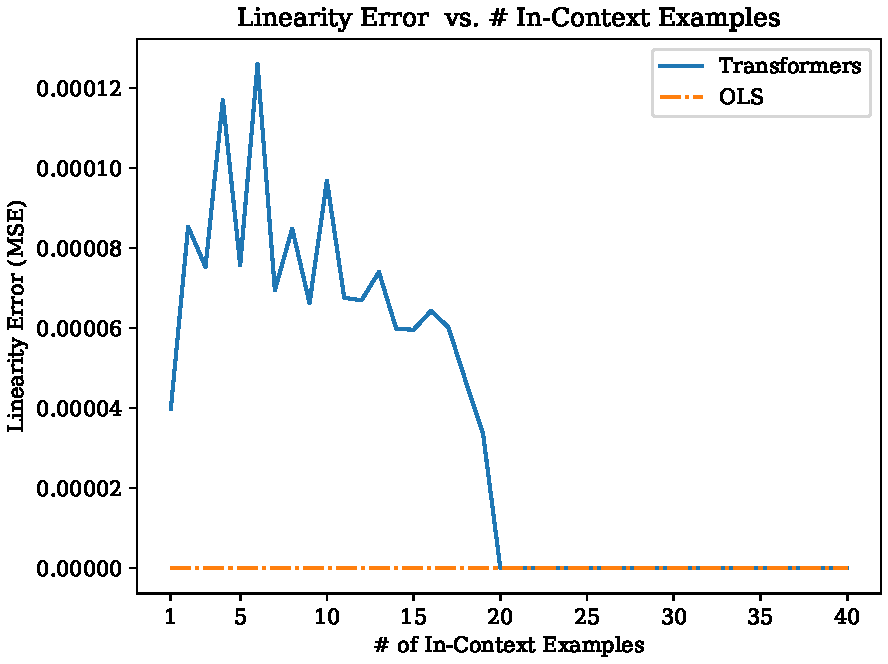
\includegraphics[width=0.6\linewidth]{Figures/linearity_error_vs_num_examples.pdf}
    \caption{Verification of hypothesis that the Transformers induced weight vector $\bw$ lies in the span of observed examples $\{\bx_i\}$. }
    \label{fig:higher_order}
\end{figure}
